\documentclass{mypaper}

\title{Manual til \texttt{svg2ais} og \texttt{plotais}}
\author{Kristian Kjærgaard}
\date{\today}

\usepackage{tikz}

\begin{document}

\maketitle

Her skal der stå en forklaring til fremgangsmåden i programmet. De
ting, jeg ikke selv er helt med på, skal fremgå her.

Ting, der skal dokumenteres:

\begin{itemize}
\item Afstandsfunktionen i Line dst underscore line
\item Algoritmen til at optimere afstanden skal pædagogiseres
\end{itemize}

Sådan gør jeg: Indlæs figuren. Hvert element er en ``Shape''.

\begin{figure}[htbp]
  \centering
  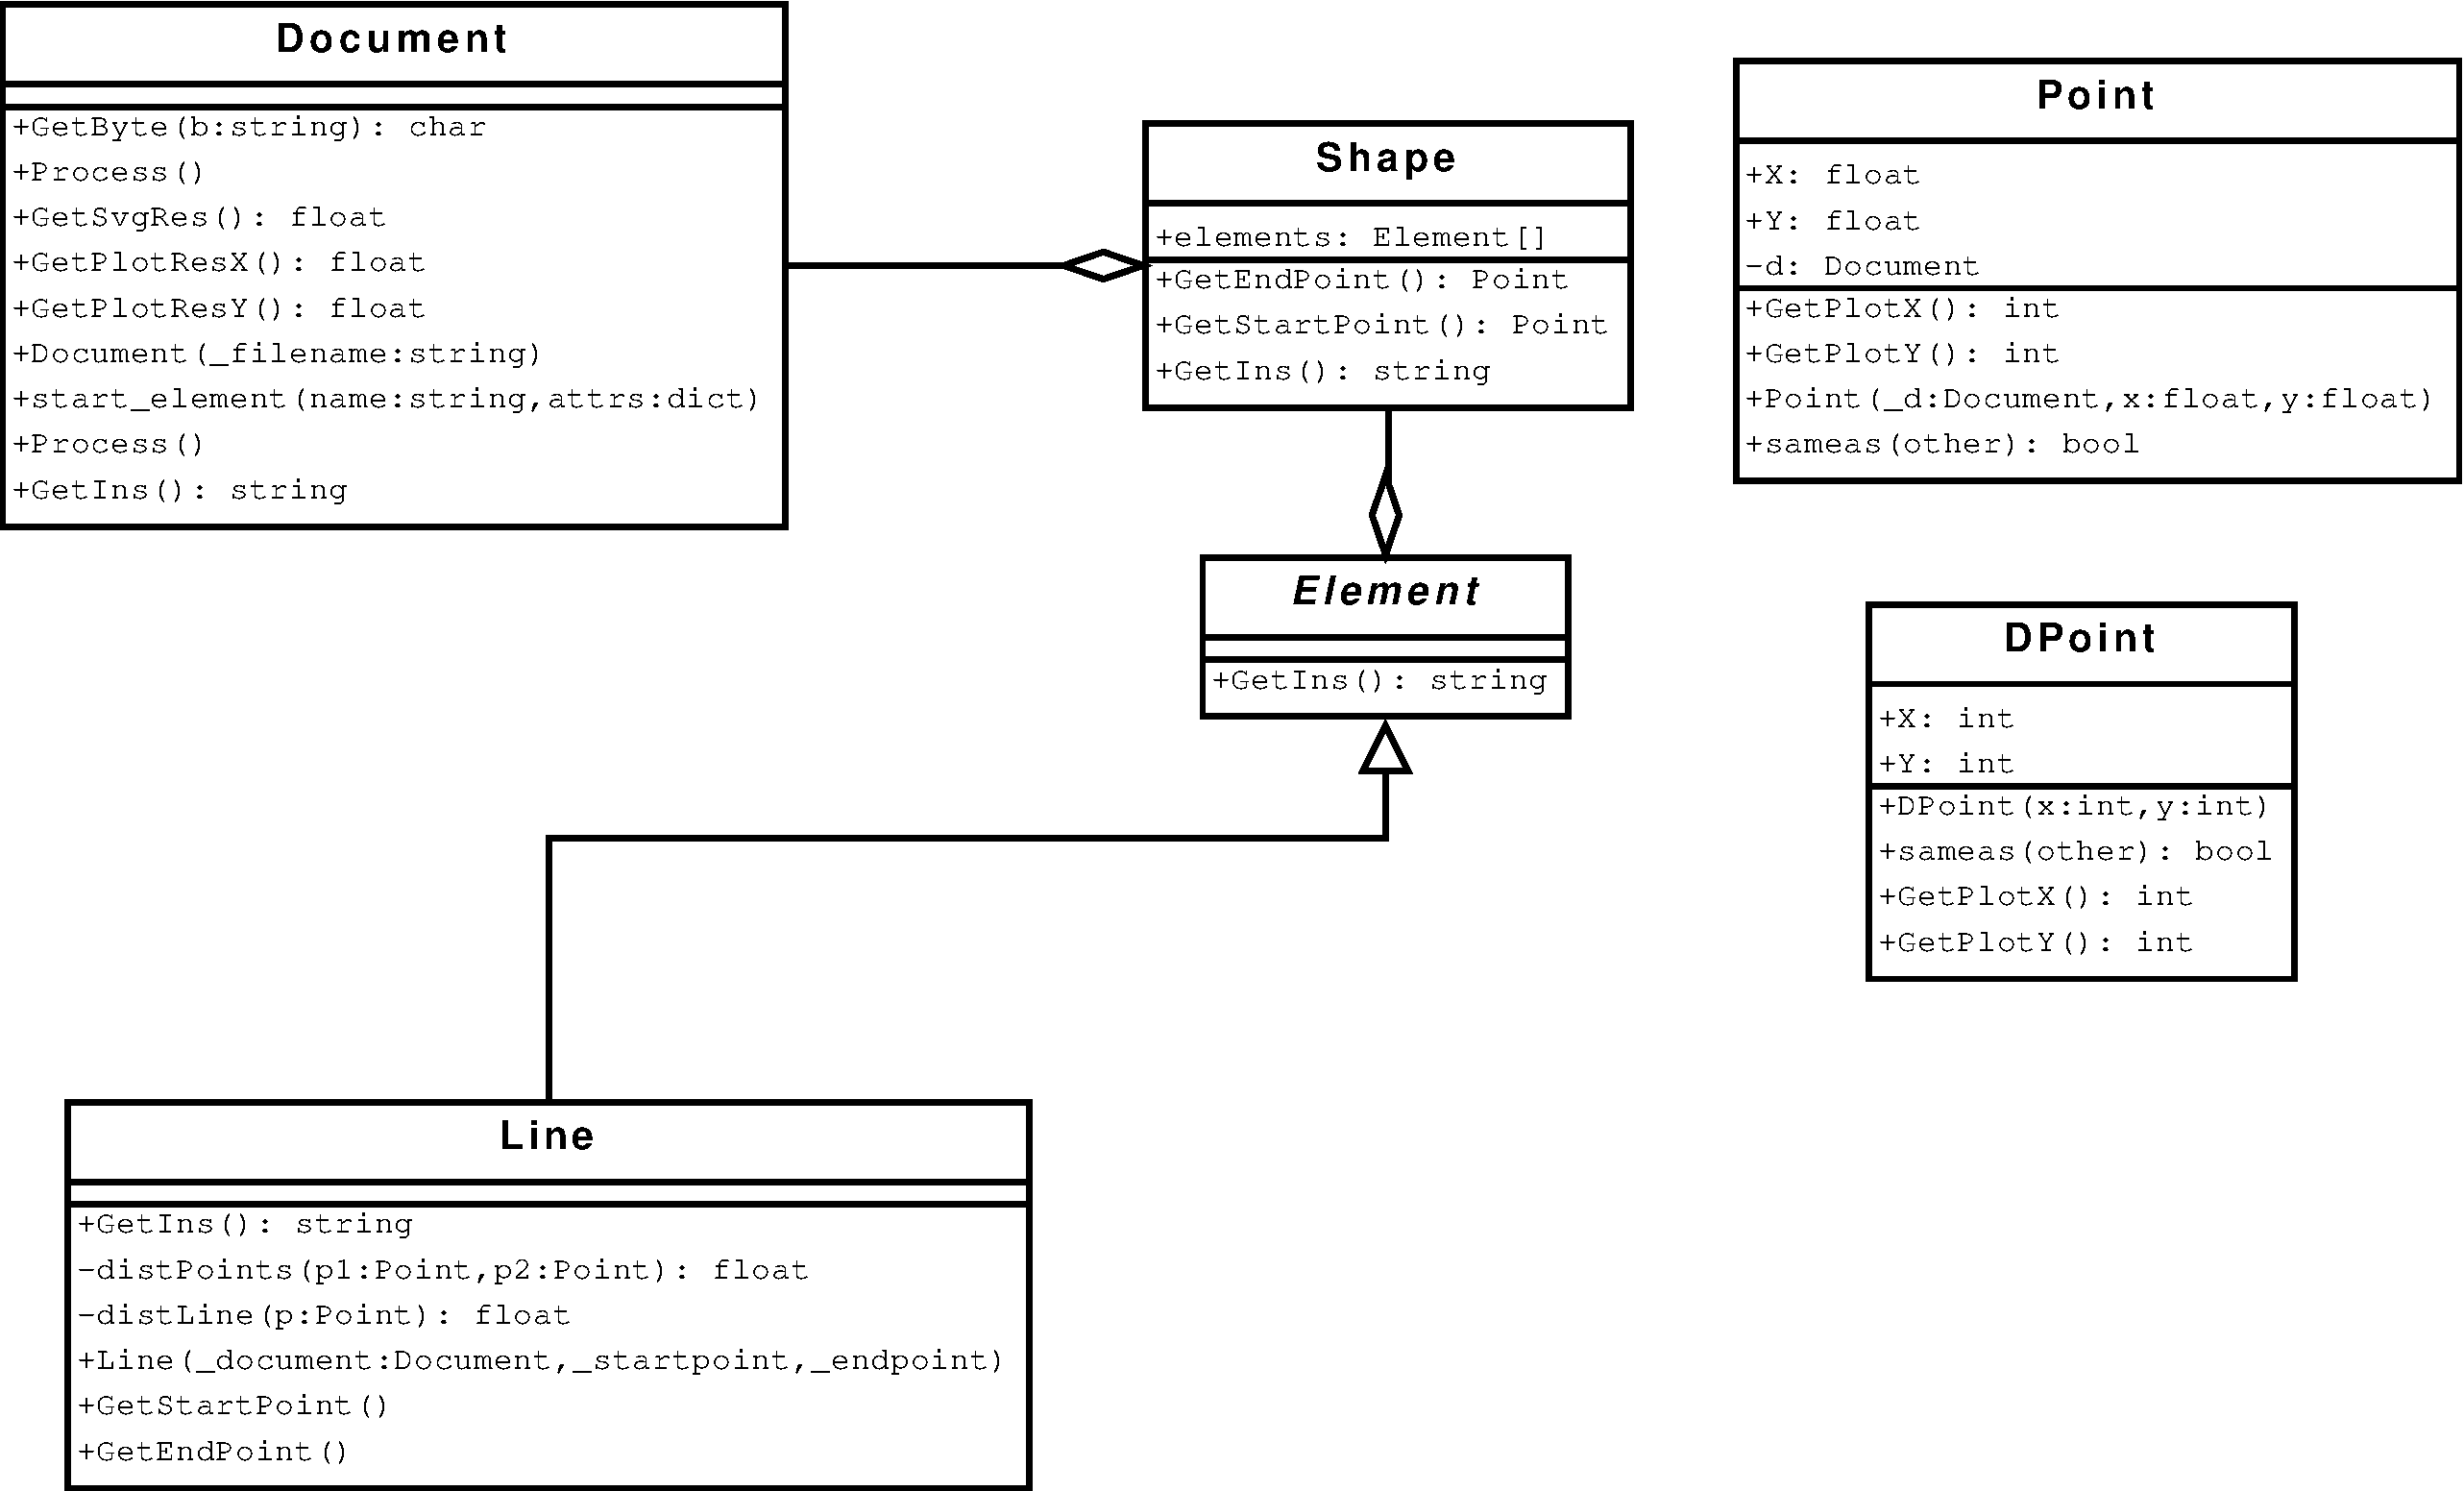
\includegraphics[width=\textwidth]{./obj-oversigt}
  \caption{Oversigt over objekter}
  \label{fig:obj-oversigt}
\end{figure}


\end{document}

%%% Local Variables:
%%% mode: latex
%%% End: